\section*{Plan de trabajo}
    En cuanto al objetivo de  simulación del proceso es necesario  contar  con el software de Aspen  plus 10.0 además datos importantes como el modelado adecuado para satisfacer los parámetros necesarios que exige el simulador. Se necesita parámetros como flujos de entrada,temperatura de operación, presión de operación, composición de las corrientes de entrada y de salida además el modelo termodinámico. Los equipos cuya información es necesaria son:\\

        \begin{enumerate}
            \item Separador flash
            \item Reactor
            \item Intercambiadores de calor
            \item Torre de absorción
            \item Torres de destilación
        \end{enumerate}

    Los cuales los podemos encontrar en los distintas referencias de este trabajo.

    Para cumplir el objetivo de simular el proceso es necesario  iniciar un nuevo proyecto en blanco en Aspen 10.0, ingresar los componentes que se utilizaran en el desarrollo de la simulación, en este caso serán  necesarios Alcohol isopropilico ($C_3H_8O$), acetona ($C_3H_6O$ ), hidrógeno ($H_2$) y agua ($H_2O$), los cuales se ingresaran en el área de \textit{components} de la izquierda superior, además  se podrá añadir un nombre de reconocimiento de cada componente en este trabajo  para dar seguimiento a la simulación se dará el ID de \textit{ IPA},\textit{ ACETONE},\textit{ WATER} e \textit{ HYDROGEN}, tal
    como se muestra en la \textit{Figura \ref{fig:componentes}}.
        \begin{figure}[H]
            \centering
            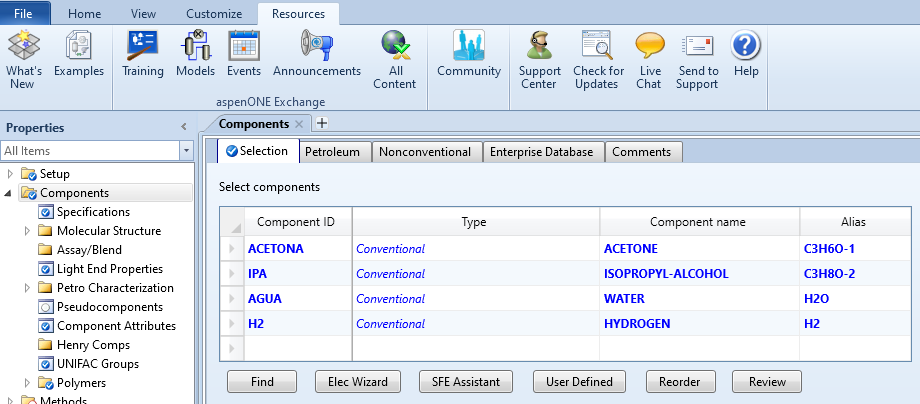
\includegraphics[scale =0.5]{images/Paso _1.PNG}
            \caption{Vista de Aspen Plus donde se introducen los componentes del proceso.}
            \label{fig:componentes}
        \end{figure}
    El siguiente paso es seleccionar el método con el que se va a trabajar, según la literatura  el método idóneo es UNIQUAC \cite{article}. El método anterior  toma en cuenta el tamaño molecular  y las diferencias de forma además de un termino residual que toma en cuenta las interacciones moleculares \cite{smith1997introduccion}, por lo tanto se especifica en la izquierda superior en el área de \textit{Methods} se selecciona UNIQUAC como en la \textit{Figura \ref{fig:Modelotermodinamico}}
        \begin{figure}[H]
            \centering
            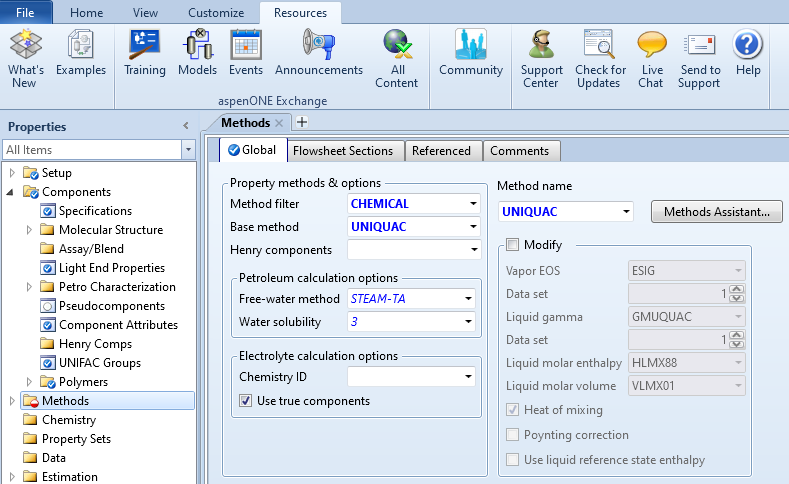
\includegraphics[scale=0.5]{images/Paso_2.PNG}
            \caption{Vista de Aspen Plus donde se muestra la selección del modelo termodinámico adecuado al proceso. Aquí se elige el modelo termodinámico UNIQUAC.}
            \label{fig:Modelotermodinamico}
        \end{figure}

    El área para  para insertar los reactores, a la izquierda inferior en el área \textit{simulation}\\ en el cual podemos escoger  entre diferentes tipos como RCSTR, Rplug, RBatch entre otros (ver\textit{ Figura \ref{fig:reactor}}).
        \begin{figure}[H]
            \centering
            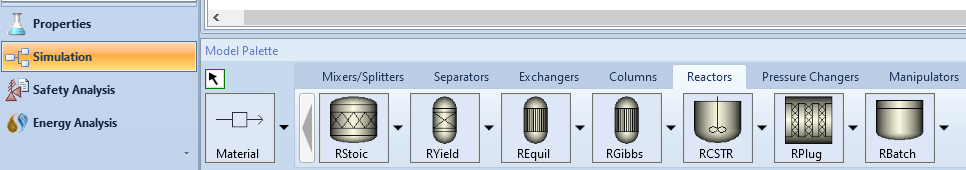
\includegraphics[scale=0.5]{images/Paso_3.PNG}
            \caption{Vista de Aspen Plus para la selección del reactor adecuado al proceso.}
            \label{fig:reactor}
        \end{figure}
    Para agregar la reacción en la sección de
    \textit{Reactions} en la cual agregaremos la reacción en ambos sentidos por ser reversible
        \begin{figure}[H]
            \centering
            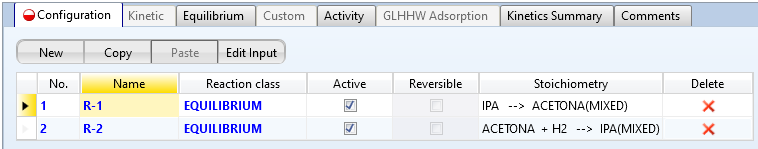
\includegraphics[scale=0.5]{images/Paso_4.PNG}
            \caption{Vista de Aspen Plus para la selección de parámetros cinéticos. Aquí seleccionamos si nuestra reacción es reversible o irreversible.}
            \label{fig:Parametrocineticos}
        \end{figure}
    Para agregar las columnas de destilación así como en el reactor, en la parte inferior  donde están las operaciones unitarias (ver\textit{ Figura \ref{fig:reactor}}) se selecciona  la pestaña de \textit{Columns} las columnas de destilación  y se llenan los datos necesarios como lo es la presión de operación que la literatura marca de 1 atm, la relación de reflujo que es de 2.78  y las distintas etapas necesarias así como la etapa  en la que se alimenta. En el proceso de Turton la primera columna tiene 67 etapas y se alimenta en la 54, para la segunda la columna tiene un total de 20 y se alimenta en la etapa 16 \cite{article}.
